\setcounter{figure}{0}

\section{9th April 2023: How does Easter bring us hope?}
\subsection*{Text: Luke 24:1-12}
  \begin{quote}
    [1] But on the first day of the week, at early dawn, they went to the tomb, taking the spices they had prepared. [2] And they found the stone rolled away from the tomb, [3] but when they went in they did not find the body of the Lord Jesus. [4] While they were perplexed about this, behold, two men stood by them in dazzling apparel. [5] And as they were frightened and bowed their faces to the ground, the men said to them, “Why do you seek the living among the dead? [6] He is not here, but has risen. Remember how he told you, while he was still in Galilee, [7] that the Son of Man must be delivered into the hands of sinful men and be crucified and on the third day rise.” [8] And they remembered his words, [9] and returning from the tomb they told all these things to the eleven and to all the rest. [10] Now it was Mary Magdalene and Joanna and Mary the mother of James and the other women with them who told these things to the apostles, [11] but these words seemed to them an idle tale, and they did not believe them. [12] But Peter rose and ran to the tomb; stooping and looking in, he saw the linen cloths by themselves; and he went home marveling at what had happened.
  \end{quote}
\subsection*{Notes}
\begin{itemize}
  \item{The tomb was empty.  The resurrection of Jesus is central to our
  Christian faith.  His death was necessary, but so was His resurrection; if
  He had not been resurrected, then His death had no meaning. One compelling piece of evidence for the resurrection was how the disciples went from being cowards to being courageous witnesses of the faith. What could be the reason why? The most plausible reason was that they did indeed see the risen Christ!}
  \item{The resurrection of Jesus guarantees the resurrection of all who are Christians, since Jesus is the first-fruits of those who had been risen from the dead (first fruits implies more fruit to come). Since the resurrection is an event that happened in our world, the effects of the resurrection is not just for the future (when we will be raised), but has very present implications for us too. Four points for today:
  \begin{itemize}
    \item{Resurrection and sin.}
    \item{Resurrection and sanctification.}
    \item{Resurrection and service.}
    \item{Resurrection and suffering.}
  \end{itemize}
  }
  \item{From 1 Corinthians 15:17,20, we see that if Christ had not been raised, our faith is in vain. In contrast, because Christ is risen, we can have full assurance that our sins are fully paid for. The resurrection of Christ implies that the penalty for sin has been fully paid for. As Paul says, the wages of sin is death, and since Jesus took on the penalty of our sin, He must die on the cross. But how do we know that our sins are fully paid for? We know because Jesus resurrection from the dead tells us that our sins have really been paid for. But does this mean that we can sin freely? This leads to the second point.}
  \item{As Paul says, in Romans 6:4, the resurrection of Jesus gives us the
  power to live new lives despite our fallen human nature.  The power that
  raised Jesus from the dead is the same power that sanctifies us.  Hence,
  since it is certain that Jesus was raised, we can have certainty that we as
  Christians will be sanctified.  But some of us will say, ``but I still
  struggle with sin!  What does this mean then?'' The answer is the ``already
  but not yet'' existence of the Kingdom of God!  Jesus' incarnation
  inaugurated the kingdom of God.  And at Jesus' resurrection, He confirmed
  the existence of the kingdom of God.  So right now, the Kingdom of God is
  in our midst.  Hence similarly for us, as John Stott says, ``the already
  means more confidence that anyone can be changed, that any enslaving habit
  can be overcome.  But on the other hand, our fallen nature remains in us
  and will never be elimimnated until the fullness of the kingdom arrives.
  The not yet means we needs more patience and understanduing with growing
  persons, it means not to be condescending nor impatient with lapses and
  failures.  ''.  Or more simply, the resurrection of Christ breaks the power
  of sin, so that we have the ability, despite our fallen nature, to offer up
  our lives to God as our acceptable spiritual worship, though it might be
  still imperfect.  And we can have the confidence that as we continue to
  live by the Spirit, we will \textbf{asymptotically} approach perfection in
  this life.  }
  \item{Next, as Paul says in 1 Corinthians 15:24, because Christ is risen,
  our work for the Lord is not in vain.  This ``work of the Lord'' refers not
  just to Christian ministry, but it also refers to the work we do in the
  marketplace.  One question; is the earth going to be replaced or renewed at
  the second coming of Christ and at the great and final resurrection?  If
  the answer is that the earth will be ``replaced'', then no real work we do
  on earth matters except the saving of souls.  But if the answer is that the
  earth will be ``renewed'', then our marketplace work is also significant.
  Everything that is true, and good, and beautiful in the work that we do in
  the marketplace will be used by God in the renewing of the new creation.
  In whatever we do, as long as we do it for the glory of God, it can be
  considered the work of the Lord.}
  \item{Lastly, as Paul says, the resurrection of Christ gives us hope in our
  suffering.  From 2 Corinthians 4:16-17, even though our outer body is
  wasting away, the resurrection of Christ which implies our resurrection
  means that we can look forward to an eternal weight of glory.  One
  interesting quote: ``In light of the weight of the glory of heaven, even
  the most miserable life on earth will look like one night in an
  inconvenient hotel''. It is axiomatic in Christianity that the way up is down, that the road to glory is the cross. If that is the pattern that our Savior took, going to the cross to be glorified, then that is the pattern we must take in our lives. And as Jesus said, ``take heart; I have overcome the world''. The resurrection of Jesus, which guarantees our future inheritance in heaven, gives us hope in our suffering. }
  \item{In conclusion: resurrection of Jesus leads to:
  \begin{itemize}
    \item{Forgiveness of sin.}
    \item{Power to be sanctified and to live sanctified lives.}
    \item{Purpose and meaning for our service to God, not just in Christian ministry, but also in our marketplace work.}
    \item{Hope in our suffering.}
  \end{itemize}
  }
  \item{\begin{figure}[H]
    \centering
    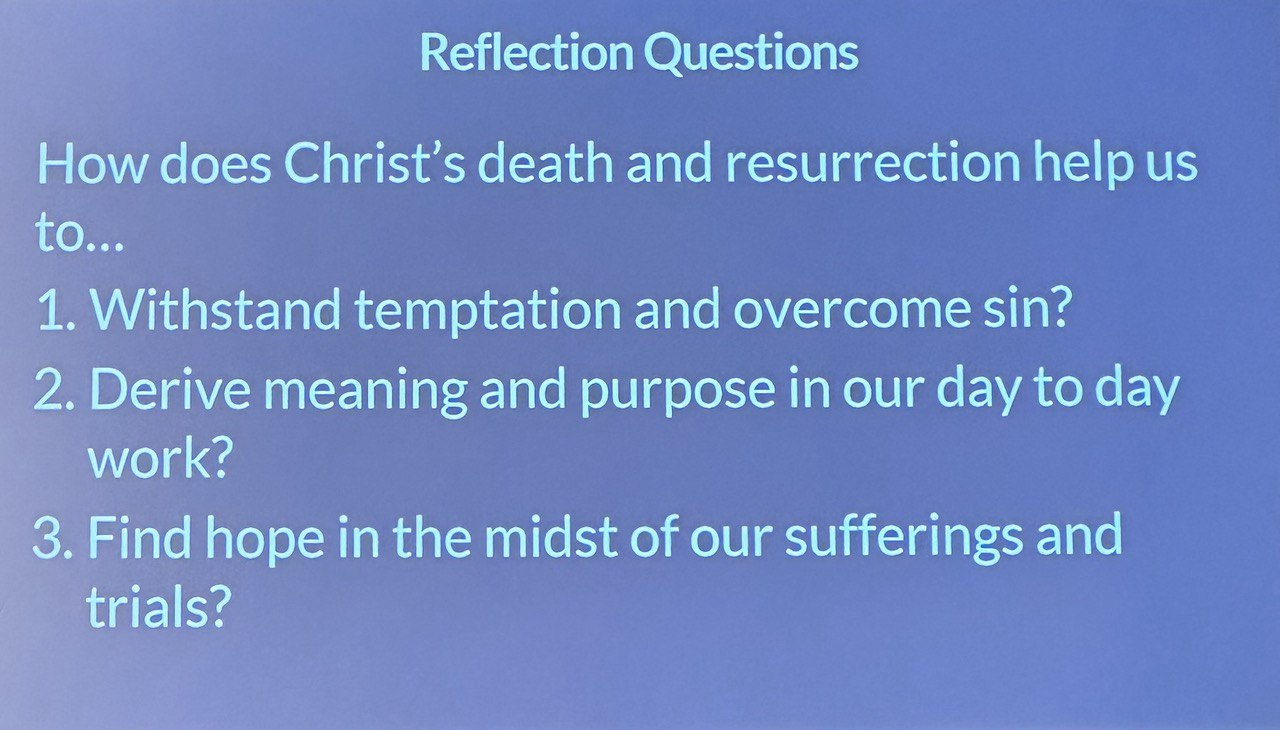
\includegraphics[width=0.8\textwidth, trim={0cm 0cm 0cm 0cm},clip]{Figures/aprilSermon2Reflections.jpg}
    \caption[]{Reflection questions for this sermon}
    % \label{}
  \end{figure}}
\end{itemize}